\documentclass{article}
\usepackage[utf8]{inputenc}
\usepackage[spanish]{babel}
\usepackage{listings}
\usepackage{subfigure}
\usepackage{graphicx}
\usepackage{url}
\usepackage{multirow}
\usepackage{multicol}
\usepackage{color}
\usepackage{booktabs}
\usepackage{float}
\usepackage{amsmath}
%\usepackage{verbatim}
\usepackage{hyperref}
\hypersetup{
    colorlinks=true,
    linkcolor=blue,
    filecolor=magenta,      
    urlcolor=cyan,
}
\usepackage[margin=3cm,twoside]{geometry} 
\setlength{\parindent}{0pt}
\setlength{\parskip}{1em}
\usepackage{fancyvrb}





\definecolor{mygreen}{rgb}{0,0.6,0}
\definecolor{mygray}{rgb}{0.5,0.5,0.5}
\definecolor{mymauve}{rgb}{0.58,0,0.82}
\lstset{ 
  backgroundcolor=\color{white},   % choose the background color; you must add \usepackage{color} or \usepackage{xcolor}; should come as last argument
  basicstyle=\footnotesize,        % the size of the fonts that are used for the code
  breakatwhitespace=false,         % sets if automatic breaks should only happen at whitespace
  breaklines=true,                 % sets automatic line breaking
  captionpos=b,                    % sets the caption-position to bottom
  commentstyle=\color{mygreen},    % comment style
  deletekeywords={...},            % if you want to delete keywords from the given language
  escapeinside={\%*}{)},          % if you want to add LaTeX within your code
  extendedchars=true,              % lets you use non-ASCII characters; for 8-bits encodings only, does not work with UTF-8
  firstnumber=1,                % start line enumeration with line 1000
  frame=single,	                   % adds a frame around the code
  keepspaces=true,                 % keeps spaces in text, useful for keeping indentation of code (possibly needs columns=flexible)
  keywordstyle=\color{blue},       % keyword style
  language=Octave,                 % the language of the code
  morekeywords={*,...},            % if you want to add more keywords to the set
  numbers=left,                    % where to put the line-numbers; possible values are (none, left, right)
  numbersep=5pt,                   % how far the line-numbers are from the code
  numberstyle=\tiny\color{mygray}, % the style that is used for the line-numbers
  rulecolor=\color{black},         % if not set, the frame-color may be changed on line-breaks within not-black text (e.g. comments (green here))
  showspaces=false,                % show spaces everywhere adding particular underscores; it overrides 'showstringspaces'
  showstringspaces=false,          % underline spaces within strings only
  showtabs=false,                  % show tabs within strings adding particular underscores
  stepnumber=1,                    % the step between two line-numbers. If it's 1, each line will be numbered
  stringstyle=\color{mymauve},     % string literal style
  tabsize=2,	                   % sets default tabsize to 2 spaces
  title=\lstname                  % show the filename of files included with \lstinputlisting; also try caption instead of title
}
\usepackage{etoolbox}
\makeatletter
\providecommand{\subtitle}[1]{% add subtitle to \maketitle
  \apptocmd{\@title}{\par {\large #1 \par}}{}{}
}
\RecustomVerbatimCommand{\VerbatimInput}{VerbatimInput}%
{fontsize=\footnotesize,
	%
	frame=lines,  % top and bottom rule only
	framesep=2em, % separation between frame and text
	rulecolor=\color{mygreen},
	%
	label=\fbox{\color{black} prueba.txt},
	labelposition=topline,
	%
	commandchars=\|\(\), % escape character and argument delimiters for
	% commands within the verbatim
	%commentchar=*        % comment character
}
\renewcommand{\theenumi}{\roman{enumi}}
\newtheorem{teor}{Teorema}
\makeatother
 \title{Tarea 11 de Modelos Probabilistas Aplicados}
\subtitle{Convolución, $\chi^2$, covarianza}
\author{5271}
\date{\today}

\begin{document}

\maketitle
\section{Introducción}
En este documento se presentan los resultados del análisis de varias propiedades y conceptos de la convolución, $\chi^2$ y covarianza de forma analítica, así como los resultados alcanzados numéricamente mediante simulación. Para la simulación se utiliza lenguaje R \cite{R}.
\section{Convolución}
Una convolución es un operador matemático que transforma dos funciones $f_1$ y $f_2$ en una tercera función $f_c$ que representa la magnitud en la que se superponen $f_1$ y una versión trasladada e invertida de $f_2$. Para el caso discreto se tiene la expresión:

$\begin{array}{rcl} f_c &=& f_1 \ast f_2 \\
& \\
          f_c(i) &=& \sum_j f_1(j) \times f_2(i - j) \end{array}$.
          
Y para el caso continuo se cuenta con la siguiente ecuación:

$(f \ast g)(z) = \displaystyle\int_{-\infty}^\infty f(z - y) \times g(y) \text{d} y =
	      \displaystyle\int_{-\infty}^\infty f(z - x) \times g(x)
	      \text{d} x.$
\subsection{Aplicaciones}
 La convolución tiene muchas aplicaciones prácticas como son:
 \begin{itemize}
     \item Procesamiento de imágenes.
     \item Filtrado de señales.
     \item Multiplicación de polinomios.
     \item Procesamiento de audio.
     \item Inteligencia artificial.
     \item Óptica.
     \item Teoría de la probabilidad.
     \item Mercado financiero.
 \end{itemize}
 
\paragraph{Teoría de la probabilidad:} Si se considera una situación en la que se tienen dos variables aleatorias independientes,  $X$ e $Y$, con funciones de densidad de probabilidad $f$ y $g$ respectivamente. Y se desea calcular la función de densidad ($X+Y$), podemos usar la convolución de $f$ y $g$. Por lo que se puede calcular la suma de cualquier número de variables independientes. Esto es importante porque muchas de las distribuciones estándar se caracterizan por patrones de convolución simples, lo que significa que podemos encontrar sus funciones de densidad de probabilidad mediante convolución.

Para realizar una prueba numérica de lo antes mencionado se utilizan los valores de rendimiento del oro y del platino obtenidos del sitio \textit{Yahoo!finanzas} en la liga: \href{https://es.finance.yahoo.com/materias-primas}{https://es.finance.yahoo.com/materias-primas}. Los valores de rendimientos fueron calculados a partir de los datos obtenidos como el valor de cierre menos el valor de apertura, el mismo es una variable aleatoria. Se pretende calcular la probabilidad conjunta de las variables $X$ (oro) e $Y$ (platino), para lo cual se utiliza la función \textit{convolve} de la librería de R que utiliza la transformada rápida de Fourier para calcular la convolución de dos secuencias. En la figura \ref{fig:1} de la página \pageref{fig:1} se puede observar los resultados obtenidos. 

\begin{figure}
\centering
\subfigure[Histograma de densidad de la variable aleatoria $X$]{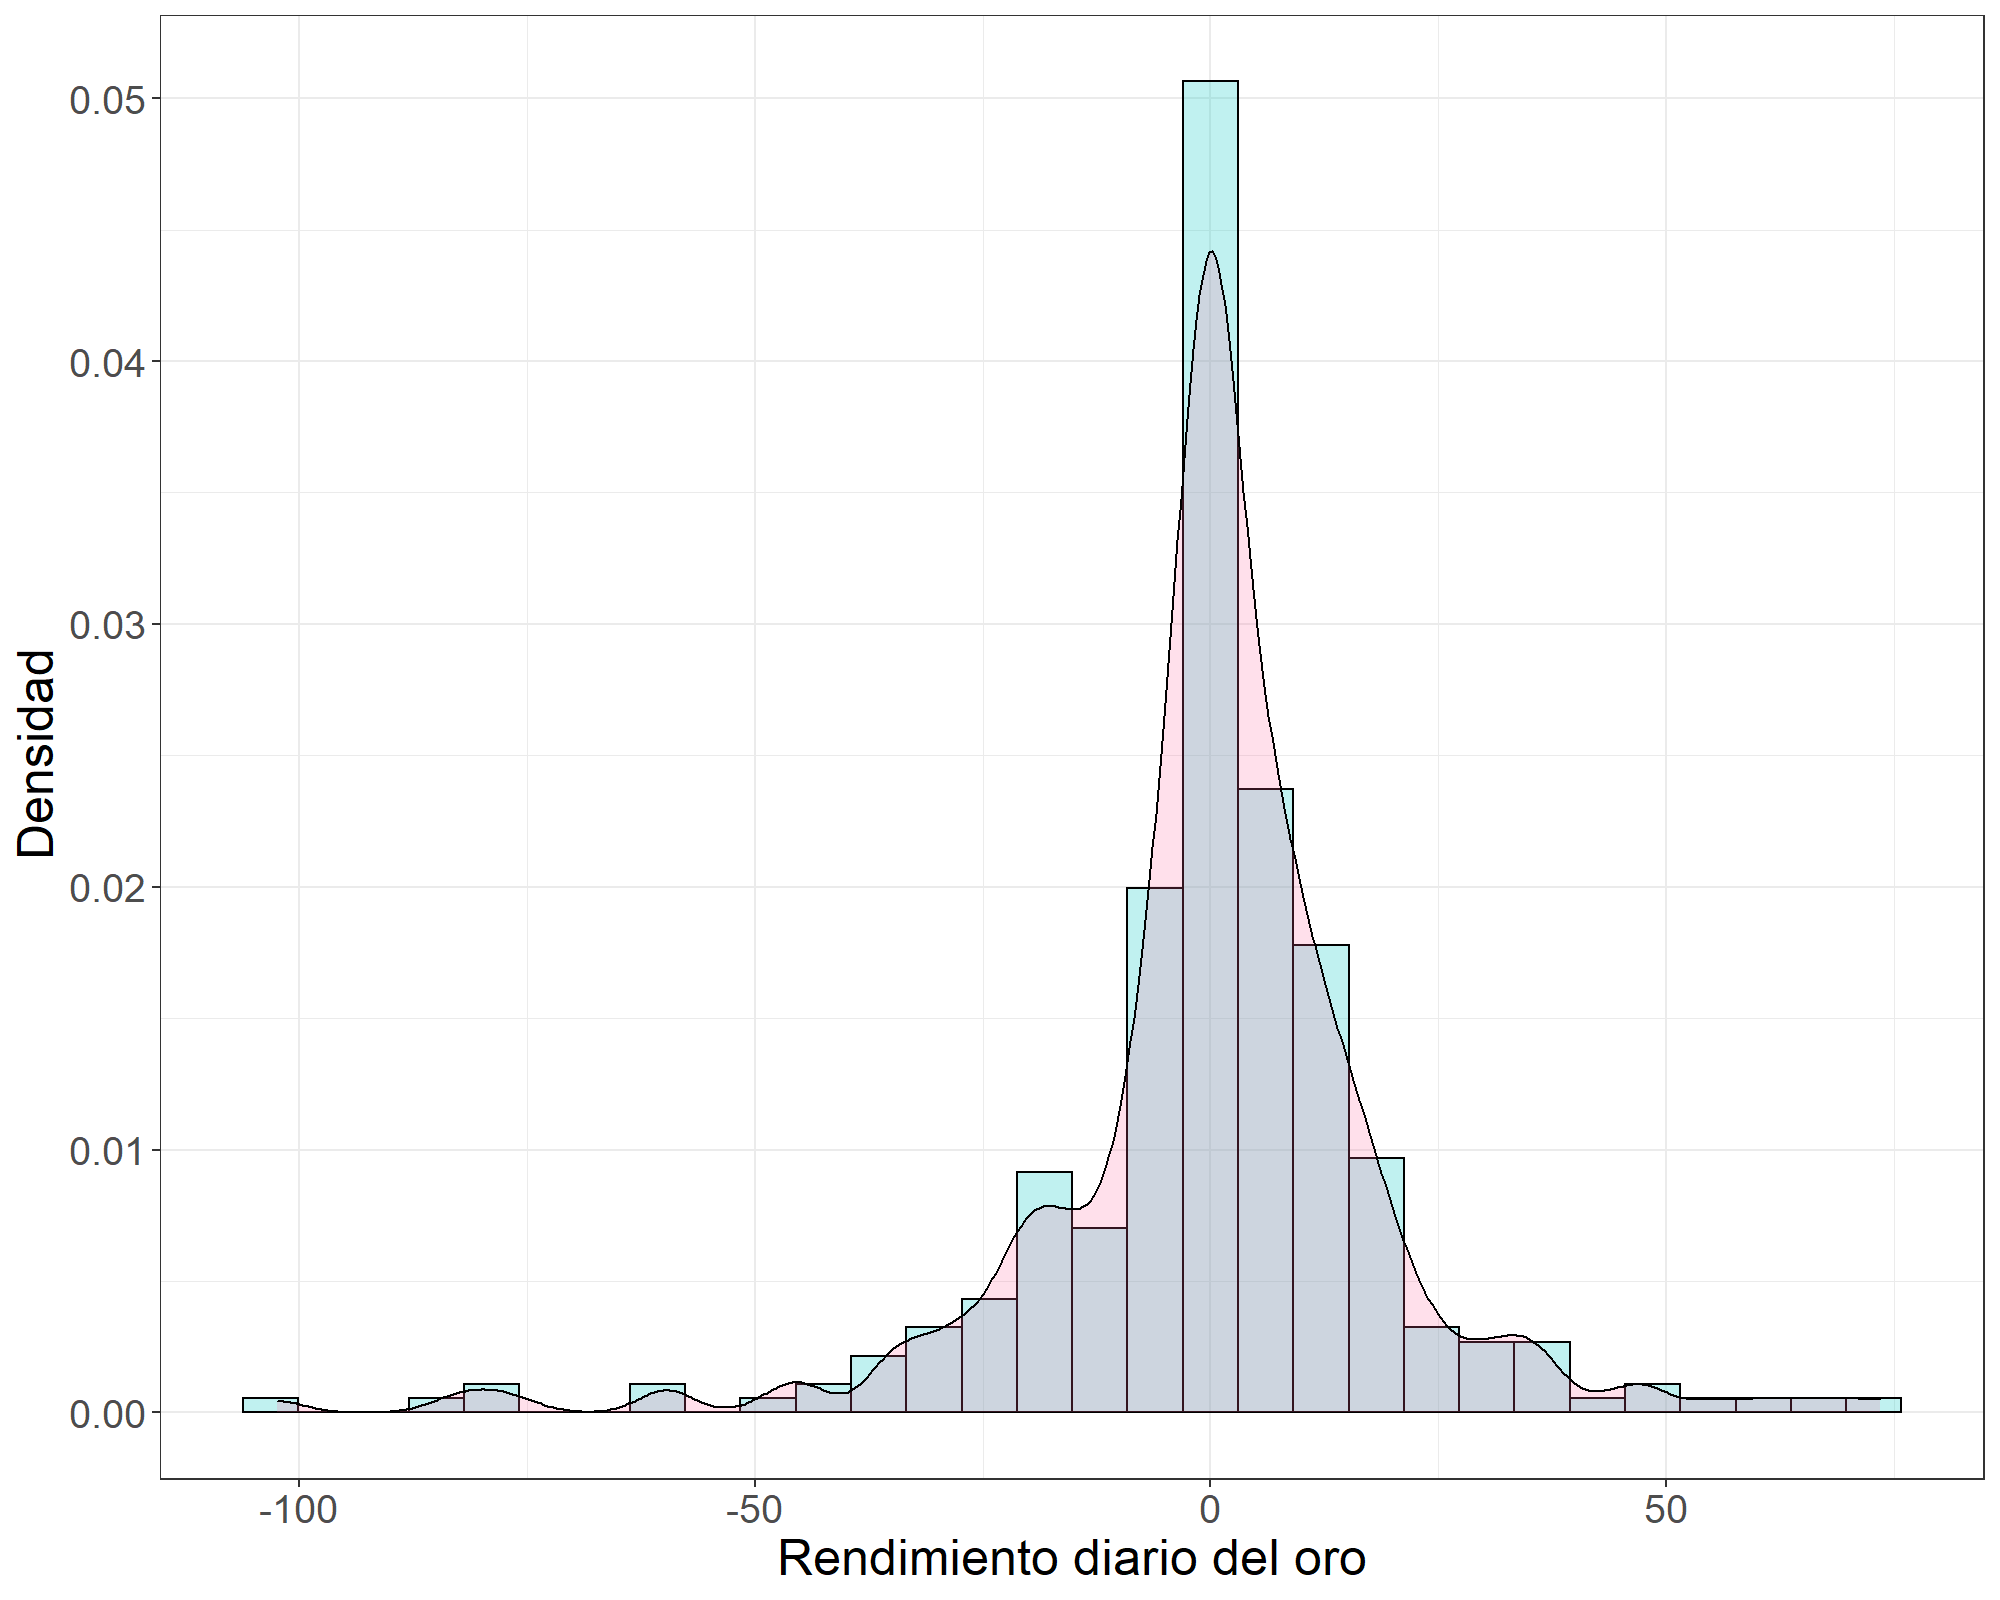
\includegraphics[scale=0.30]{figuras/oro.png}}
\label{fig:a}
\centering
\subfigure[Histograma de densidad de la variable aleatoria $Y$]{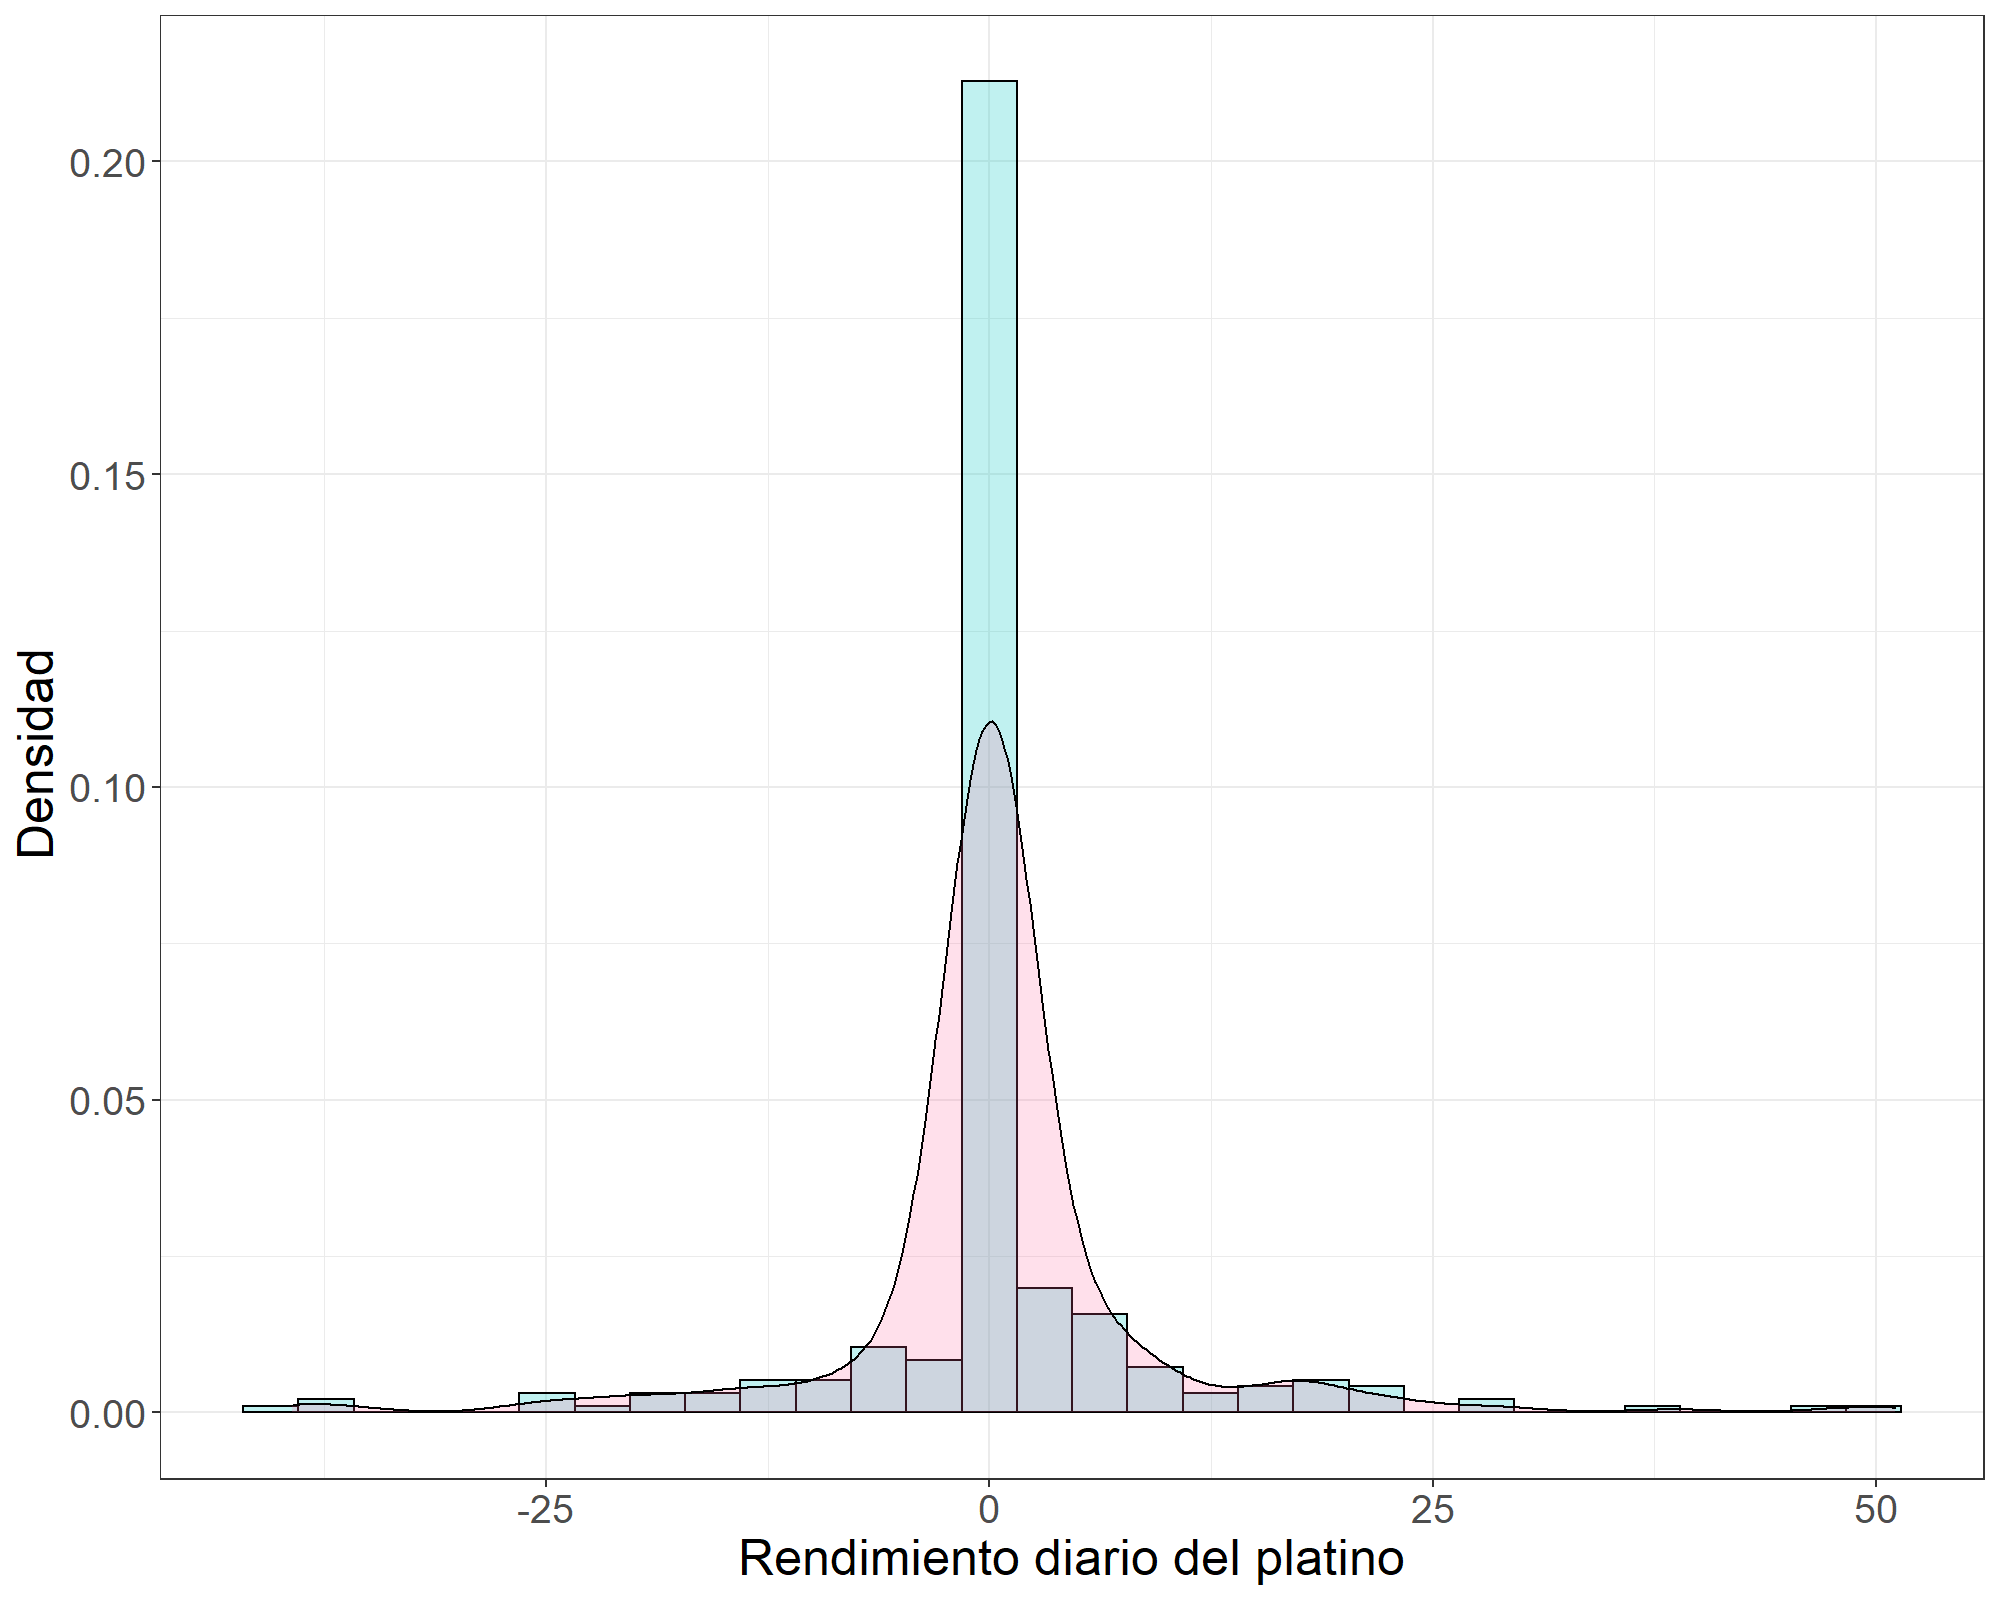
\includegraphics[scale=0.30]{figuras/plata.png}}
\label{fig:s}
\centering
\centering
\subfigure[Histograma de densidad conjunta de las variable aleatoria $X$ e $Y$]{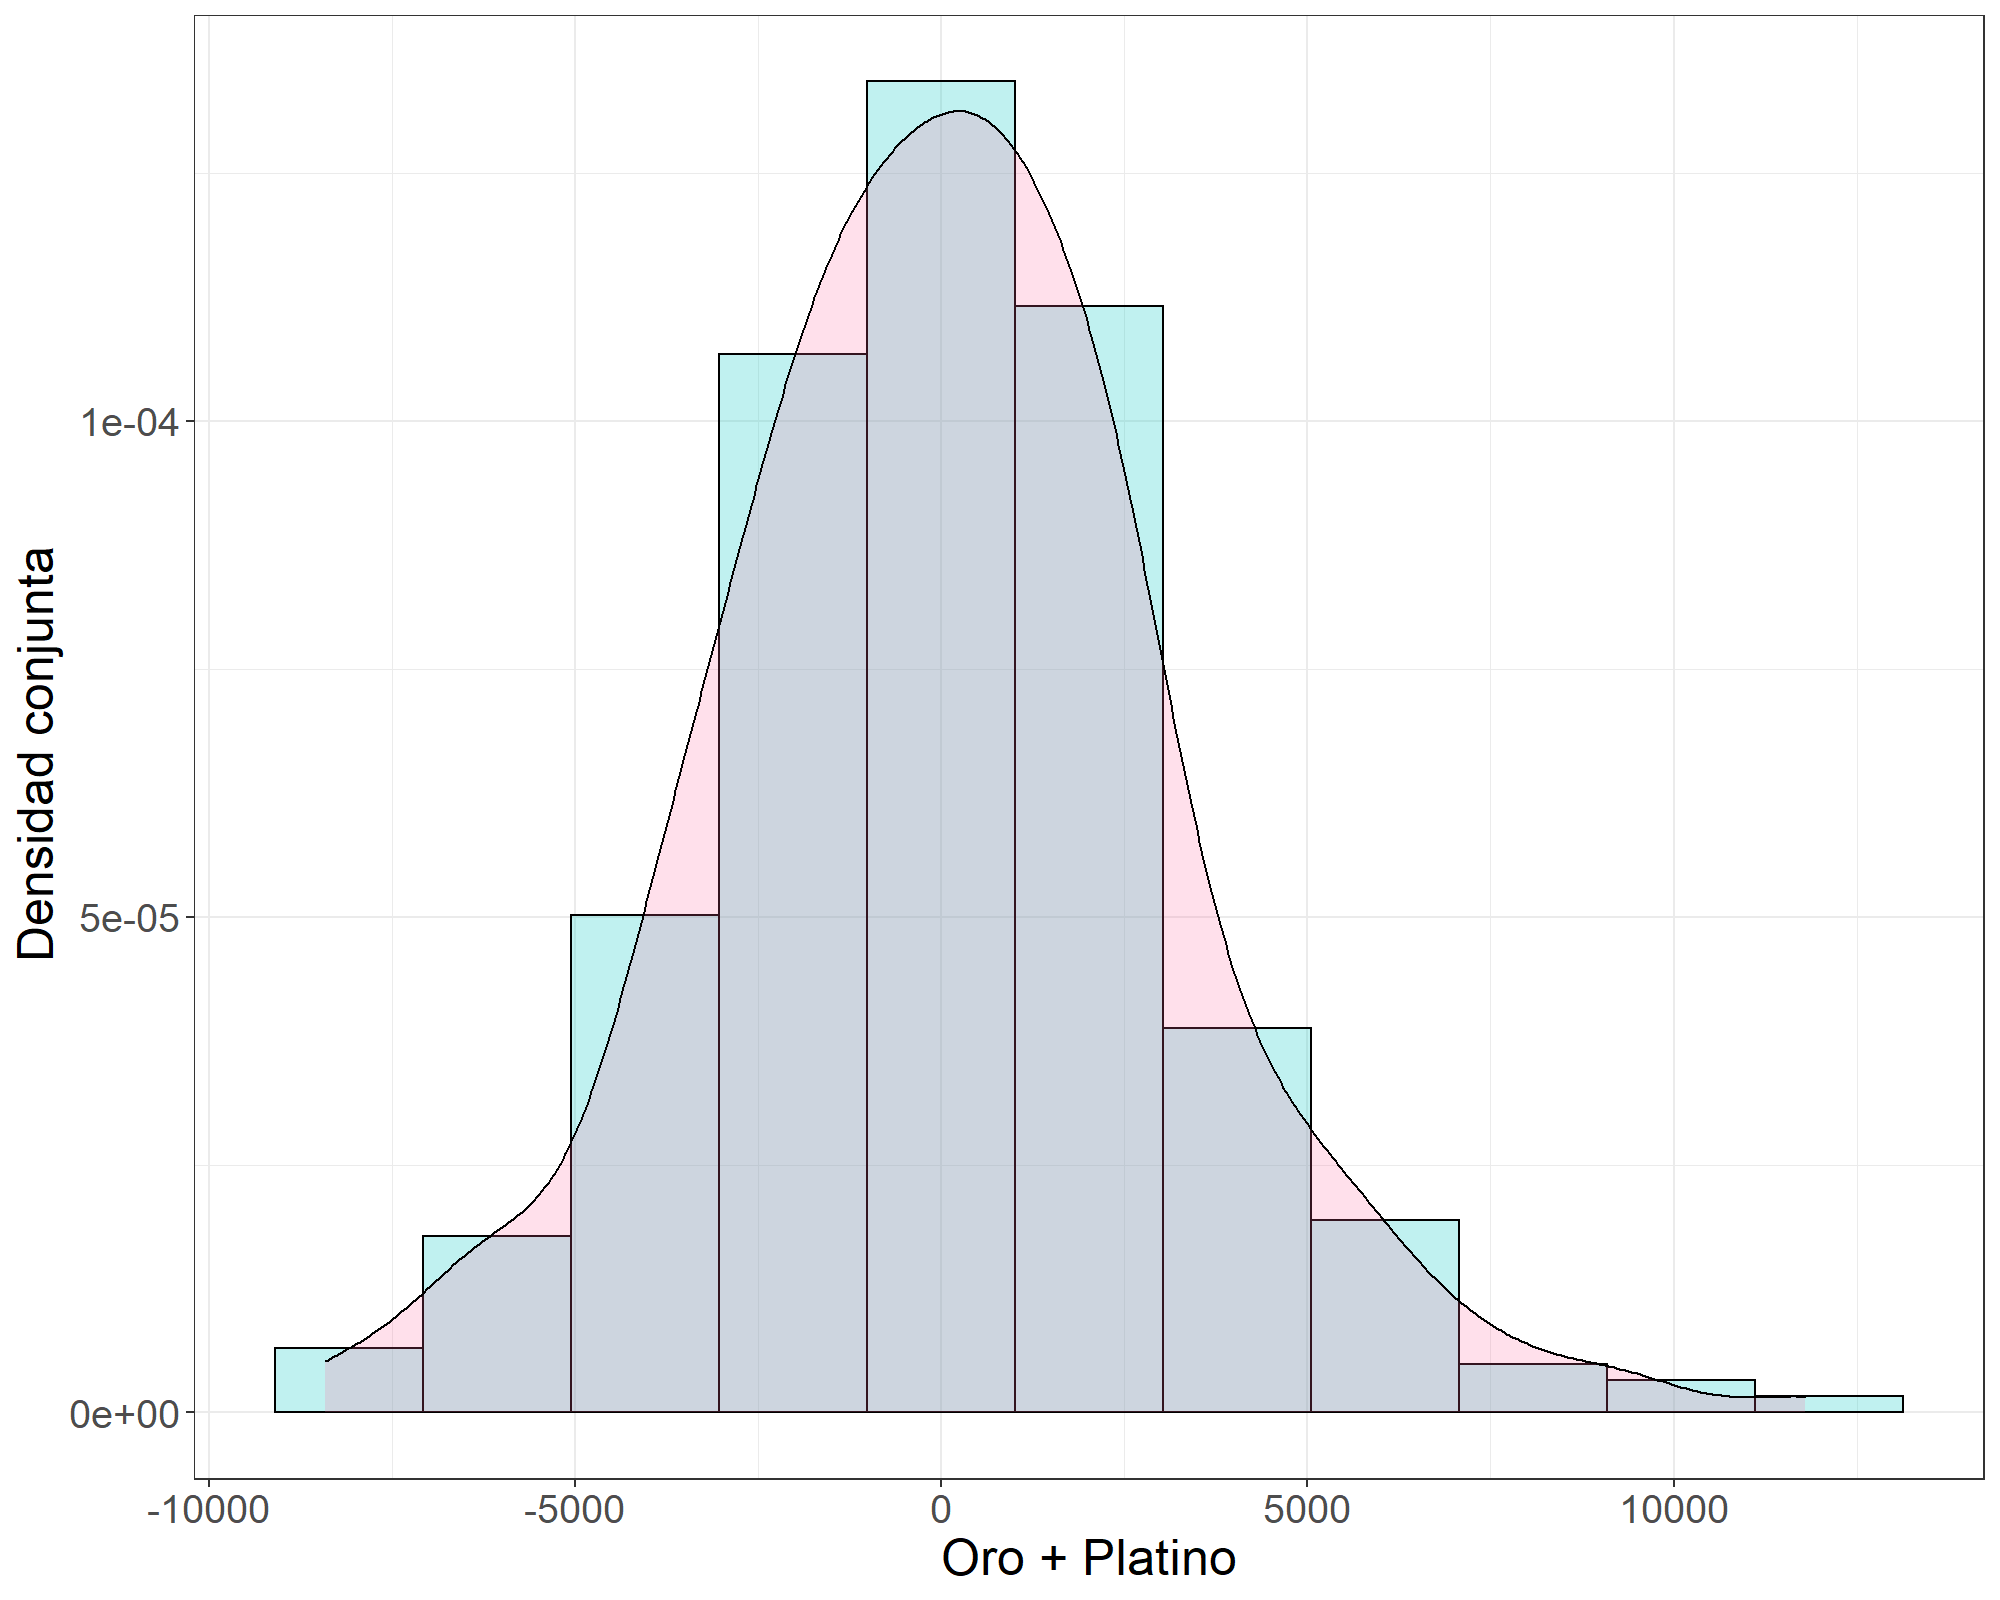
\includegraphics[scale=0.30]{figuras/plataoro.png}}
\label{fig:d}
\centering
\caption{Histogramas de la variables aleatorias $X$ e $Y$ y su convolución}
\label{fig:1} 
\end{figure}
 En la figura \ref{fig:a} y \ref{fig:s} de la página \pageref{fig:1}, muestran un comportamiento similar a la distribución normal, aunque no es tan evidente como en la \ref{fig:d} que muestra que la distribución de la convolución de las variables se distribuye normalmente. Lo anterior se corrobora aplicando la prueba de Shapiro-Wilk, que calcula un W estadístico que prueba si una muestra aleatoria $x{1}, x_{2},...,x_{n}$ proviene de una distribución normal. Al aplicar la prueba con un valor del estadístico $W=0.99112$ y un valor $p=0.0643>0.05$ no se tiene suficiente evidencia para rechazar la hipótesis nula, que plantea que la variable sigue una distribución normal, esto se puede afirmar con un intervalo de confianza del 95\%.
 \VerbatimInput{shap.txt}


\section{Chi cuadrada ($\chi^{2}$)}
 La distribución $\chi^{2}$ se utiliza  para examinar tiene si un conjunto de datos presenta una diferencia estadísticamente significativa de lo que se espera. Para la misma necesitamos conocer la distribución que se espera ver y las frecuencias observadas de cada valor posible.
 Para el caso de estudio en este trabajo, se tiene el valor de densidad de empaquetamiento de seis tipos de figuras (triángulos,rectángulos, cuadrados,pentágonos, cuadriláteros mixtos y hexágonos) en un contenedor circular. Los valores de densidad se clasifican en tres categorías:
 \begin{itemize}
     \item Malos (densidad $\leq 0.40$).
     \item Buenos ($0.40>$ densidad $\leq 0.70$).
     \item Muy buenos (densidad $> 0.70$).
 \end{itemize}
 Esta clasificación se puede ver en el cuadro \ref{tab:4} de la página \pageref{tab:4}, teniendo esto se plantea la hipótesis nula ($H_{0}$) que el tipo de figura no afecta en que la densidad de empaquetamiento sea mala, buena o muy buena. Para probar esta $H_{0}$ se realiza la prueba de \textit{chisq.test} de la librería de R como se muestra a continuación.
 \VerbatimInput{chi.txt}
 Con el estadístico $\chi^{2} = 16.171$ y un valor $p = 0.0003 < 0.05$, se tiene suficiente evidencia para rechazar la $H_{0}$, por lo que se puede decir que el tipo de figura si influye en la calidad de la densidad de empaque, con un intervalo de confianza del 95\%. 
\begin{table}[H]
  \centering
  \caption{Clasificación de los resultados de densidad para cada figura}
    \begin{tabular}{lrrrr}
    \toprule
    Figuras & \multicolumn{1}{l}{Malos} & \multicolumn{1}{l}{Buenos} & \multicolumn{1}{l}{Muy buenos} & \multicolumn{1}{l}{\textbf{Total}} \\
    \midrule
    Triángulo  & 1     & 20    & 14    & \textbf{35} \\
    Rectángulo & 2     & 22    & 11    & \textbf{35} \\
    Cuadrados & 5     & 20    & 10    & \textbf{35} \\
    Pentágono & 7     & 16    & 7     & \textbf{30} \\
    Cuadrilátero mix & 7     & 23    & 5     & \textbf{35} \\
    Hexágono & 5     & 24    & 6     & \textbf{35} \\
    \textbf{Total} & \textbf{27} & \textbf{125} & \textbf{53} & \textbf{205} \\
    \bottomrule
    \end{tabular}%
  \label{tab:4}%
\end{table}%

\section{Covarianza}
En probabilidad y la estadística, la covarianza es una medida del grado en que dos variables aleatorias (X, Y) varían conjuntamente entorno a los valores de sus medias. Si las variables tienden a mostrar un comportamiento similar, la covarianza es positiva. En el caso contrario, cuando son inversamente proporcionales, la covarianza es negativa. Por lo que se puede carcular como se muestra en la ecuación \ref{eq:1} de la página \pageref{eq:1}.
\begin{equation}\label{eq:1}
	  \text{Cov}[X, Y] = E[(X - \mu_X)(Y -\mu_Y)]. 
\end{equation}

\subsection{Propiedades de la covarianza}
En esta sección se comprobará numéricamente y analíticamente dos de las propiedades de la covarianza. 
\paragraph{Primera:} Se tiene:
\begin{equation}\label{eq:2}
\text{Cov}[aX + b, cY + d] = ac  \cdot \text{Cov}[X, Y]  
\end{equation}
Para demostrar numéricamente la igualdad planteada en la ecuación \ref{eq:2} de la página \pageref{eq:2}, se crean diez pares de variables aleatorias $X$ con distribución normal e $Y = \left( \frac{X}{2}\right)*\frac{d}{a}$ como se puede ver en el cuadro \ref{tab:1} de la página \pageref{tab:1}. Posteriormente se les asignan valores a las constantes $a, b, c, d$. Lo anterior se realiza con el código \ref{cod:1} que se muestra a continuación.

\begin{center}
\lstinputlisting[ language=R, firstline=2, lastline=16]{R/Tarea11.R}
\label{cod:1}
\end{center}

\begin{table}[H]
  \centering
  \caption{Fragmento de uno de los pares de variables aleatorias $X$ e $Y$ creadas}
    \begin{tabular}{rrr}
    \toprule
          & \multicolumn{1}{c}{X} & \multicolumn{1}{c}{Y} \\
    \midrule
    1     & 1.41293 & 1.20647 \\
    2     & -0.44490 & 0.27755 \\
    3     & 1.02916 & 1.01458 \\
    4     & 0.54957 & 0.77478 \\
    5     & -1.35893 & -0.17946 \\
    54    & -0.13546 & 0.43227 \\
    55    & 1.06661 & 1.03331 \\
    56    & 0.65222 & 0.82611 \\
    57    & 1.04822 & 1.02411 \\
    58    & -1.37364 & -0.18682 \\
    \bottomrule
    \end{tabular}%
  \label{tab:1}%
\end{table}%
\begin{table}[H]
  \centering
  \caption{Resultados de ambos miembros de la ecuación \ref{eq:2}}
    \begin{tabular}{rrrc}
    \toprule
          & \multicolumn{1}{l}{M. izquierdo(M.i)} & \multicolumn{1}{l}{M. derecho(M.d)} & \multicolumn{1}{l}{M.i  =  M.d} \\
    \midrule
    1     & 10.28066 & 10.28066 & Si \\
    2     & 6.25041 & 6.25041 & Si \\
    3     & 14.60058 & 14.60058 & Si \\
    4     & 15.01817 & 15.01817 & Si \\
    5     & 6.16484 & 6.16484 & Si \\
    6     & 16.68462 & 16.68462 & Si \\
    7     & 14.00431 & 14.00431 & Si \\
    8     & 16.71537 & 16.71537 & Si \\
    9     & 7.37975 & 7.37975 & Si \\
    10    & 3.11481 & 3.11481 & Si \\
    \bottomrule
    \end{tabular}%
  \label{tab:2}%
\end{table}%
Como se observa en el cuadro \ref{tab:2} de la página \pageref{tab:2}, para todas las variables aleatorias $X$ e $Y$ creadas los valores del miembro izquierdo de la ecuación \ref{eq:2} son iguales al miembro derecho de dicha ecuación. De esta manera queda demostrado numéricamente la igualdad planteada. Para esta comprobar la igualdad de manera analítica es conveniente recordar las dos propiedades siguientes.

Sea a y c dos constantes,
\begin{equation}\label{eq:3}
\text {Cov}(a X,Y)= a \cdot \text{Cov}(X,Y)
\end{equation}
\begin{equation}
\text {Cov}(X+c,Y)= \text{Cov}(X,Y).
\label{eq:4}
\end{equation}
 Desarrollando el lado izquierdo de la ecuación \ref{eq:2} se tiene:
 \begin{equation}
  \begin{array}{cll}
   \text{Cov}[aX + b, cY + d]    & = ac  \cdot \text{Cov}[X+b, Y+d],&\text{por  la propiedad \ref{eq:3}}, \\
      
                        & = ac  \cdot \text{Cov}[X, Y],&\text{por propiedad \ref{eq:4}}.
  \end{array}
 \end{equation}
\paragraph{Segunda:} Se tiene:

\begin{equation}
    \text{Var}[X + Y] = \text{Var}[X] + \text{Var}[Y] + 2\cdot  \text{Cov}[X, Y]
    \label{eq:6}
\end{equation}
Para la comprobación numérica de la igualdad \ref{eq:6} de la página \pageref{eq:6}, se utiliza el código \ref{cod:2}, los valores de las variables aleatorias y las constantes tienen las mismas características que en el caso anterior.
\begin{center}
\lstinputlisting[ language=R, firstline=31, lastline=45]{R/Tarea11.R}
\label{cod:2}
\end{center}

\begin{table}[H]
  \centering
  \caption{Resultados de ambos miembros de la ecuación \ref{eq:6}}
    \begin{tabular}{rrrc}
    \toprule
          & \multicolumn{1}{l}{M. izquierdo(M.i)} & \multicolumn{1}{l}{M. derecho(M.d)} & \multicolumn{1}{l}{M.i  =  M.d} \\
    \midrule
    1     & 2.49469 & 2.49469 & Si \\
    2     & 2.23400 & 2.23400 & Si \\
    3     & 2.44015 & 2.44015 & Si \\
    4     & 2.20168 & 2.20168 & Si \\
    5     & 2.37420 & 2.37420 & Si \\
    6     & 2.40887 & 2.40887 & Si \\
    7     & 2.17660 & 2.17660 & Si \\
    8     & 1.95016 & 1.95016 & Si \\
    9     & 2.60644 & 2.60644 & Si \\
    10    & 1.98039 & 1.98039 & Si \\
    \bottomrule
    \end{tabular}%
  \label{tab:3}%
\end{table}%
En los resultados que se muestran en el cuadro \ref{tab:3} de la página \pageref{tab:3}, queda comprobado de forma numérica la igualad planteada en la ecuación \ref{eq:6}. Para la corporación analítica de ecuación en cuestión, no apoyamos de las expresiones siguientes:
\begin{equation}
 \text{Var}[X]= E[X^{2}] - E[X]^{2}.  
\end{equation}
\begin{equation}
 \text{Cov}(X,Y)= E[XY] - E[X]E[Y].  
\end{equation}
 Desarrollando el lado izquierdo de la ecuación \ref{eq:6} se tiene:
 \begin{equation}
     \begin{array}{cl}
       \text{Var}[X + Y]    & = E[(X+Y)^{2}] - E[X+Y]^{2} \\
                            &  \\
                            & = E[(X+Y)^{2}] - E[X+Y]^{2} \\
                            &  \\
                            & = E[X^{2}]- E[X]^{2} + E[Y^{2}]- E[Y]^{2} + 2\cdot E[XY]  - 2\cdot E[X]E[Y]  \\ 
                            &  \\
                            & = \text{Var}[X] + \text{Var}[Y] + 2 ( E[XY]- E[X]E[Y])\\ 
                            &  \\
                            & = \text{Var}[X] + \text{Var}[Y] +2\text{Cov}(X,Y).
     \end{array}
 \end{equation}
 
 El código general se encuentra disponible en el repositorio. \href{https://github.com/Albertomnoa/Tareas_MPA/tree/master/Tarea10}{https://github.com/Albertomnoa/Tareas} \textbf{} 

   
\newpage
\bibliographystyle{plain}
\bibliography{Biblio}

\end{document}
